\documentclass[12pt,a4paper,titlepage]{article}

\usepackage[T1]{fontenc}
\usepackage[polish]{babel}
\usepackage[utf8]{inputenc}
\usepackage{lmodern}
\usepackage{graphicx}
\selectlanguage{polish}

\setlength{\parindent}{5mm} %ustawi rozmiar wcie˛cia na pocza˛tku kaz˙dego akapitu na 0mm,
\setlength{\parskip}{4mm}	%

\title{Sprawozdanie z ćwiczenia laboratoryjnego}
\date{2014}
\author{Tomasz Mikołajewski }

\begin{document}
\maketitle
\pagestyle{empty}
%\pagestyle{headings}
\tableofcontents

\section{Wprowadzenie}
Niniejszy dokument powstał w ramach przedmiotu Projektowanie Algorytmów i Metod Sztucznej Inteligencji. Jest on rezultatem przeprowadzonych ćwiczeń w laboratorium oraz pracy wykonanej w domu.


Ćwiczenie polegało na przeprowadzeniu analizy złożoności operacji wykonywanych na strukturach przechowujących dane wraz z kluczami. Podczas tekstu sprawdzano struktury: szybkiego sortowania, sortowania przez kopcowanie oraz przez scalanie. Podczas testu sprawdzane były struktury drzewa oraz tablicy z hashowaniem. Testowanie powtarzano wielokrotnie, aby uzyskać ilość danych pozwalającą na wyznaczenie przybliżonej funkcji opisującej złożoność algorytmu. 

\section{Kod programu}
Program został oparty o wcześniej stworzone pliki zawierające kod potrzebny do wykonania \textit {benchmark-u} podprogramu, czyli określenia czasu jaki potrzebny jest na jego wykonanie. Główny program zawiera funkcję otwierającą pliki z danymi oraz zapisującą rezultat operacji do pliku. Dodatkowo do programu wykonującego sprawdzenie algorytmów dodano metodę automatycznie tworzącą plik z danymi potrzebnymi do sprawdzenia algorytmu. Wszystkie ustawienia można zmieniać w pliku \textit {konfiguracja.hh}. Zdecydowanie ułatwia to prace przy analizie zadanej struktury.

Testy, które zostały przeprowadzone na strukturach to:
\begin{itemize}
\item wpisywanie danych
\item wyszukiwanie danych
\item wielokrotne wyszukiwanie danych
\end{itemize}


\section{Pomiary}
Pomiary zostały przeprowadzone na plikach o różnych wielkościach zaczynając od 300, a kończąc na 1000000 elementów. Każda ze struktur był testowany dla co najmniej 5 różnych rozmiarów problemów powtórzonych dla dziesięciu różnych plików generowamych w sposób losowy. Aby otrzymać rzetelny pomiar, każdy z testów był uśredniany, a w wypadku małych plików operacje były powtarzane 1000 krotnie w celu uzyskanie większej dokładności. Ponad to przeprowadzono również analizę różnych ustawień parametrów dla tablicy z hashowanie. 

\section{Wyniki pomiarów}
Po przeprowadzeniu serii pomiarów otrzymano wyniki przedstawione w tabelach. Na podstawie wyników utworzono wykresy zamieszczone poniżej.


\subsection{Drzewo}
Drzewo jest strukturą przechowującą oprócz danych również wskaźniki łączące pojedyncze, elementy w większą strukturę. Każdy z elementów posiada wskaźniki do elementu większego oraz mniejszego dzięki czemu możliwe jest szybkie wyszukanie odpowiedniego elementu. Dodatkowo testowane drzewo zawierało wskaźniki \textit {ojca} danego elementu, co znacząco ułatwiało usuwanie elementów.


\subsubsection{Wpisywanie danych do drzewa}
Doświadczenie zostało przeprowadzone na danych typu klucz-liczba wygenerowanych w celu sprawdzenia algorytmu. 

\begin{center}
\begin {tabular}{|c|c|c|c|c|c|}\hline
ilość elementów&1000000&600000&300000&200000&100000\\\hline
&1,59&1,08&0,46&0,36&0,18\\\hline
&1,52&0,94&0,5&0,36&0,16\\\hline
&2,27&1,13&0,5&0,37&0,19\\\hline
&1,98&1,05&0,63&0,28&0,17\\\hline
&1,97&1,29&0,49&0,41&0,16\\\hline
&1,88&1,04&0,58&0,38&0,17\\\hline
&1,67&1,14&0,51&0,34&0,19\\\hline
&1,75&1,01&0,52&0,42&0,16\\\hline
&2,15&0,78&0,44&0,31&0,17\\\hline
&1,79&1,4&0,47&0,32&0,17\\\hline
czas średni&1,857&1,086&0,51&0,355&0,172\\\hline
\end{tabular}
\end {center}
\begin{figure}[h]
\begin{center}
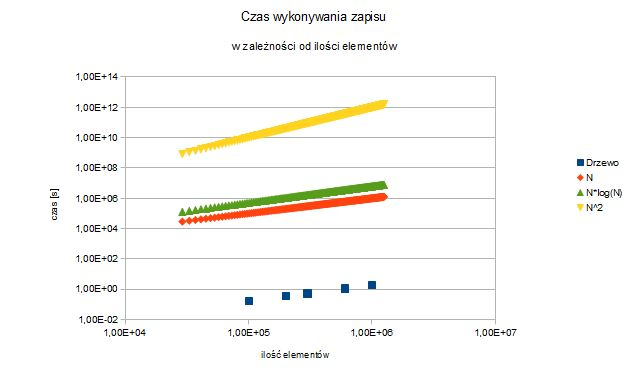
\includegraphics[scale=0.7]{wpisywanie_drzewo.jpg}
\caption{Wpisywanie do drzewa}
\end{center}
\end{figure}

\subsection{Tablica z hashowaniem}
Dane o zadanej strukturze można umieścić w tablicy z hashowaniem. Jednakże najprostsza z możliwych tablic ma wiele wad takich jak wysokie wymogi co do zajmowanej pamięci jak i konieczności nie powtarzania się elementów. Ulepszono więc tą strukturę tworząc tablicę wskaźników do początków list dwukierunkowych. Takie rozwiązanie pozwala ograniczyć wielkość zapotrzebowania na pamięć, jak również umożliwia przechowywanie kilku elementów o tym samym kluczu.
\subsubsection{Badanie wpływu parametrów tablicy z hashowaniem}
Doświadczenie przeprowadzone w celu sprawdzenia działania wpisywania elementów dla różnej początkowej wielkości struktury. Algorytm tworzący tablicę z hashowaniem sprawdza określoną ilość liter hasła i na tej podstawie przydziela odpowiedni numer komórki tablicy. Zwiększanie liczby sprawdzanych liter powoduje powiększenie tablicy. Jednakże im większa tablica tym krócej trwa odczyt i zapis. Należy więc odpowiednio dobrać wielkość tablicy dla danego problemu.  

\begin{center}
\begin {tabular}{|c|c|c|c|c|}\hline
ilość elementów&300000&100000&60000&30000\\\hline
&7,59&1,04&0,23&0,07\\\hline
&7,64&1,19&0,23&0,07\\\hline
&7,78&1,17&0,23&0,08\\\hline
&7,72&1,28&0,23&0,07\\\hline
&7,77&1,07&0,24&0,07\\\hline
&7,85&1,24&0,24&0,07\\\hline
&7,78&1,22&0,26&0,08\\\hline
&7,86&1,21&0,24&0,07\\\hline
&8,14&1,32&0,25&0,08\\\hline
&7,73&1,34&0,24&0,08\\\hline
czas średni&7,786&1,208&0,239&0,074\\\hline

\end{tabular}
\end {center}


\begin{figure}[h]
\begin{center}
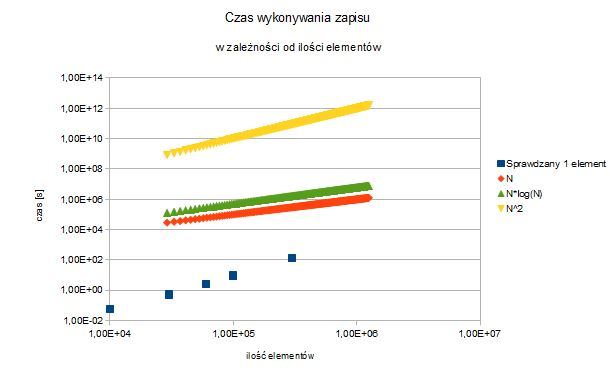
\includegraphics[scale=0.7]{1_element.jpg}
\caption{Tablica ze sprawdzanym 1 elementem}
\end{center}
\end{figure}

\begin{center}
\begin {tabular}{|c|c|c|c|c|c|}\hline
ilość elementów&300000&100000&60000&30000&10000\\\hline
&134,17&8,78&2,51&0,5&0,06\\\hline
&134,601&8,95&2,59&0,51&0,06\\\hline
&136,47&9,4&2,68&0,52&0,06\\\hline
&138,89&9,14&2,64&0,51&0,06\\\hline
&137,64&9,1&2,67&0,51&0,06\\\hline
&138,611&9,27&2,66&0,52&0,06\\\hline
&136,83&9,05&2,67&0,52&0,06\\\hline
&138,07&9,23&2,83&0,52&0,06\\\hline
&139,011&9,03&2,68&0,51&0,06\\\hline
&137,61&9,26&2,8&0,51&0,06\\\hline
czas średni&137,1903&9,121&2,673&0,513&0,06\\\hline

\end{tabular}
\end {center}


\begin{figure}[h]
\begin{center}
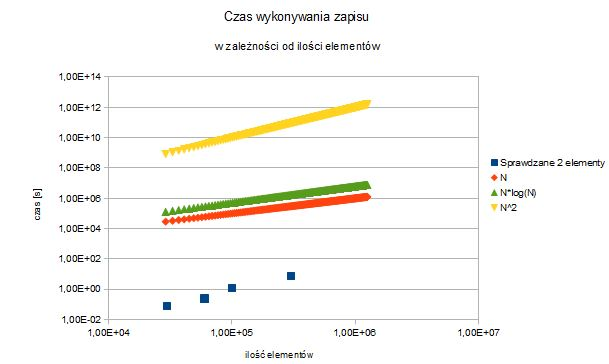
\includegraphics[scale=0.7]{2_elementy.jpg}
\caption{Tablica ze sprawdzanym 2 elementami}
\end{center}
\end{figure}

\begin{center}
\begin {tabular}{|c|c|c|c|c|c|c|c|}\hline
ilość elementów&1000000&600000&300000&200000&100000&60000&30000\\\hline
&34,64&11,05&2,15&0,92&0,249&0,109&0,047\\\hline
&34,89&11,53&2,18&0,97&0,25&0,109&0,046\\\hline
&36,07&12,286&2,2&0,94&0,25&0,125&0,062\\\hline
&35,68&11,485&2,24&1&0,25&0,124&0,047\\\hline
&35,65&11,563&2,25&0,99&0,265&0,125&0,047\\\hline
&35,27&11,667&2,32&0,95&0,265&0,109&0,062\\\hline
&36,51&11,39&2,29&0,96&0,25&0,109&0,047\\\hline
&35,93&11,304&2,37&0,97&0,25&0,125&0,047\\\hline
&36,17&11,74&2,44&1&0,265&0,124&0,047\\\hline
&35,67&11,93&2,37&0,94&0,249&0,125&0,062\\\hline
czas średni&35,648&11,5945&2,281&0,964&0,2543&0,1184&0,0514\\\hline
\end{tabular}
\end {center}


\begin{figure}[h]
\begin{center}
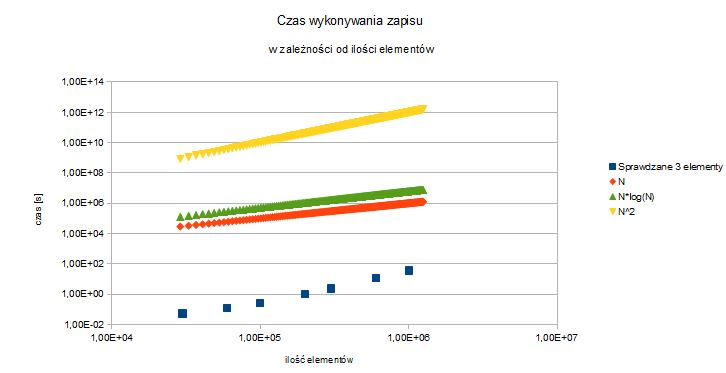
\includegraphics[scale=0.7]{3_elementy.jpg}
\caption{Tablica ze sprawdzanym 3 elementami}
\end{center}
\end{figure}

\begin{figure}[h]
\begin{center}
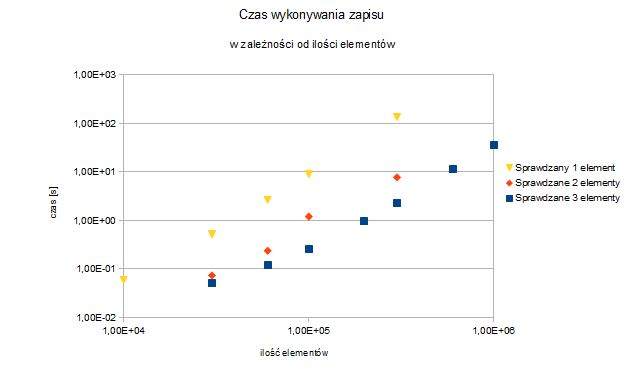
\includegraphics[scale=0.7]{porowanie_elementow.jpg}
\caption{Porównanie przypadków}
\end{center}
\end{figure}

Jak widać na zamieszczonych wykresach zwiększenie ilości sprawdzanych elementów znacząco zmniejsza czas potrzebny na wykonanie operacji zapisu N elementów. Warto jednak przeanalizować jakie wielkości pamięci są do tego potrzebne.

\begin{center}
\begin {tabular}{|c|c|}\hline
Ilość elementów& Ilość potrzebnych miejsc\\\hline 
1&32\\\hline 
2&1024\\\hline 
3&32768\\\hline 
\end{tabular}
\end {center}

\newpage
\newpage
\subsection{Porównanie struktur}
Zestawiono również tabele oraz wykresy porównujące otrzymane struktury. Przeprowadzane były dwa testy:
\begin{itemize}
\item wpisywanie danych
\item wyszukiwanie danych
\end{itemize}

Warto nadmienić że drugi z nich był wykonywany dla małych i dużych plików danych

\subsubsection{Wpisywanie danych}
Test polegał na wpisaniu danych do struktur i zmierzeniu otrzymanego czasu. Zamieszczone wykresy zostały wykonane na podstawie danych z poprzedniego punktu. Dla tablicy hashującej przyjęto, że komórka pamięci jest przydzielana na podstawie 3 pierwszych liter hasła. Reszta klucza była wykorzystywana do tworzenia listy, na którą wskazywała wcześniej wymieniona komórka.


\begin{figure}[h]
\begin{center}
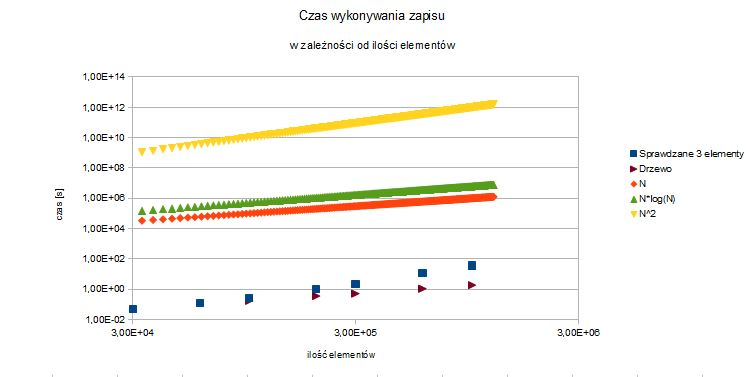
\includegraphics[scale=0.5]{porownanie_zapisu.jpg}
\caption{Porównania zapisu elementów}
\end{center}
\end{figure}

\subsubsection{Szukanie danych}
Wyszukiwanie danych w strukturach było priorytetem w przedstawianym zadaniu. Tablica hashująca została stworzon z myślą o znajdowaniu w niej elementów. Wykonano test struktur wprowadzając do nich różne ilości elementów, a następnie wyszukujące każdy z nich. Dane zebrano w tabeli.

\begin{center}
\textbf{Dane dla tablicy hashującej-duża ilość danych}
\begin {tabular}{|c|c|c|c|c|c|}\hline
ilość elementów&1000000&300000&100000&30000&10000\\\hline
&84,22&4,77&0,35&0,04&0,01\\\hline
&83,46&4,71&0,35&0,04&0,01\\\hline
&84,1&4,98&0,37&0,04&0\\\hline
&86,26&4,55&0,37&0,05&0,01\\\hline
&84,43&4,79&0,35&0,04&0,01\\\hline
&84,812&4,9&0,36&0,04&0,01\\\hline
&86,45&4,59&0,36&0,04&0\\\hline
&92,224&4,78&0,36&0,04&0,01\\\hline
&94,05&5,5&0,34&0,04&0\\\hline
&94,93&4,88&0,37&0,04&0,01\\\hline
czas średni&87,4936&4,845&0,358&0,041&0,007\\\hline
\end{tabular}
\end {center}

\begin{center}
\textbf{Dane dla tablicy hashującej - mała ilość danych}
\begin {tabular}{|c|c|c|c|c|c|}\hline
ilość elementów&10000&3000&1000&300&30000\\\hline
&0,0084&0,00212&0,00068&0,00022&0,04137\\\hline
&0,00843&0,00209&0,00067&0,00021&0,04108\\\hline
&0,00852&0,0021&0,00067&0,00021&0,041\\\hline
&0,00862&0,00211&0,00066&0,00021&0,040271\\\hline
&0,0085&0,00209&0,00068&0,00021&0,04106\\\hline
&0,00867&0,00212&0,00067&0,00021&0,04134\\\hline
&0,00878&0,00212&0,00067&0,0002&0,04192\\\hline
&0,00867&0,0021&0,00067&0,0002&0,04352\\\hline
&0,00843&0,0021&0,00066&0,0002&0,04306\\\hline
&0,00888&0,00211&0,00067&0,0002&0,04406\\\hline
czas średni&0,00859&0,002106&0,00067&0,000207&0,0418681\\\hline

\end{tabular}
\end {center}

\begin{center}
\textbf{Dane dla drzewa - duża ilość danych}
\begin {tabular}{|c|c|c|c|c|c|}\hline
ilość elementów&1000000&300000&100000&30000&10000\\\hline
&235,904&19,36&2,34&0,12&0,02\\\hline
&233,268&11,35&3,3&0,12&0,02\\\hline
&189,6&12,76&1,33&0,22&0,02\\\hline
&363,89&21,83&1,68&0,24&0,03\\\hline
&344,247&12,82&1,14&0,12&0,02\\\hline
&267,445&12,76&1,37&0,16&0,02\\\hline
&315,416&13,99&2,17&0,27&0,02\\\hline
&387,758&17,881&4,32&0,26&0,03\\\hline
&320,019&15,47&1,61&0,14&0,02\\\hline
&234,381&18,34&1,39&0,11&0,02\\\hline
czas średni&289,1928&15,6561&2,065&0,176&0,022\\\hline

\end{tabular}
\end {center}

\begin{center}
\textbf{Dane dla drzewa - mała ilość danych}
\begin {tabular}{|c|c|c|c|c|c|}\hline
ilość elementów&10000&3000&1000&300&30000\\\hline
&0,02472&0,00511&0,00118&0,0003&0,200744\\\hline
&0,02257&0,00453&0,00129&0,00029&0,15868\\\hline
&0,02205&0,00824&0,00129&0,0003&0,2058\\\hline
&0,02617&0,00443&0,00128&0,00029&0,156263\\\hline
&0,02929&0,00434&0,00115&0,00029&0,254449\\\hline
&0,03218&0,00467&0,00126&0,00029&0,183621\\\hline
&0,02826&0,00471&0,00141&0,0003&0,158521\\\hline
&0,03993&0,00454&0,00124&0,00031&0,220654\\\hline
&0,02602&0,00497&0,00125&0,00031&0,297539\\\hline
&0,0238&0,00578&0,00158&0,00031&0,138306\\\hline
czas średni&0,027499&0,005132&0,001293&0,000299&0,1974577\\\hline

\end{tabular}
\end {center}


\begin{figure}[h]
\begin{center}
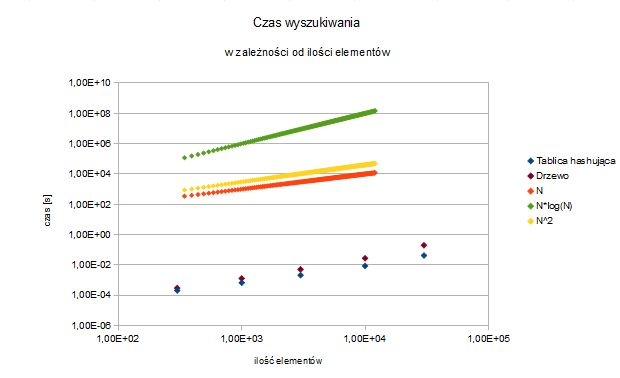
\includegraphics[scale=0.5]{wyszukiwanie_male.jpg}
\caption{Porównanie struktur dla małych ilości danych}
\end{center}
\end{figure}


\begin{figure}[h]
\begin{center}
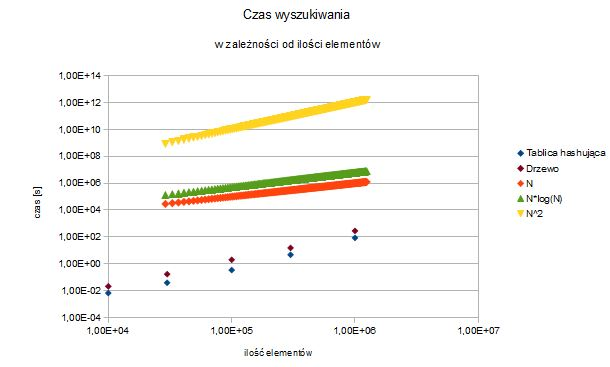
\includegraphics[scale=0.5]{wyszukiwanie_duze.jpg}
\caption{Porównanie struktur dla dużych ilości danych}
\end{center}
\end{figure}


\newpage
\section{Wnioski}
Na podstawie danych i wykresów można wyciągnąć następujące wnioski:
\begin{itemize}
\item wpisywanie danych do tablicy hashującej jest klasy 1(N) dla N mniejszego niż wielkość tablicy (nie uwzględniając wersji pesymistycznej). Dla ilości elementów większej od wcześniej wymienianej algorytm zmienia swoja złożoność i dla bardzo dużej ilości elementów posiada złożoność liniową.
\item wpisywanie danych do drzewa posiada złożoność obliczeniową klasy log(N)
\item wykorzystanie drzewa jest korzystniejsze dla wpisywanie danych w większej ilości niż około 100000
\item szybkość zapisu dla tablicy z hashowanie można dobrać za pomocą odpowiedniego doboru wielkości tablicy
\item zwiększenie ilości sprawdzanych liter znacząco wpływa na wzrost zajmowanej pamięci w wypadku tablicy z hashowaniem
\item dla niewielkiej ilości danych wyszukiwanie w tablicy z hashowaniem ma złożoność 1(N), dla większych ilości danych osiąga złożoność log(N)
\item wyszukiwanie elementów w drzewie posiada złożoność log(N) bez względu na ilość elementów
\item tablica z hashowaniem okazała się efektywniejsza podczas wyszukiwania elementów
\item przy szukaniu elementów nie występujących w strukturze efektywniejsza jest tablica hashująca, ponieważ wyszukiwanie odbywa się tylko na jednej z list i to tylko do momentu, aż klucze nie staną się większe od poszukiwanego. W wypadku drzewa należy przeprowadzić przeszukiwanie aż do szczytowej gałęzi.
\end{itemize}

\end{document}
